\documentclass[tikz,border=7pt]{standalone}
\usepackage[utf8]{inputenc}
\usepackage[OT4,plmath]{polski}
\usepackage{amsmath}
\begin{document}
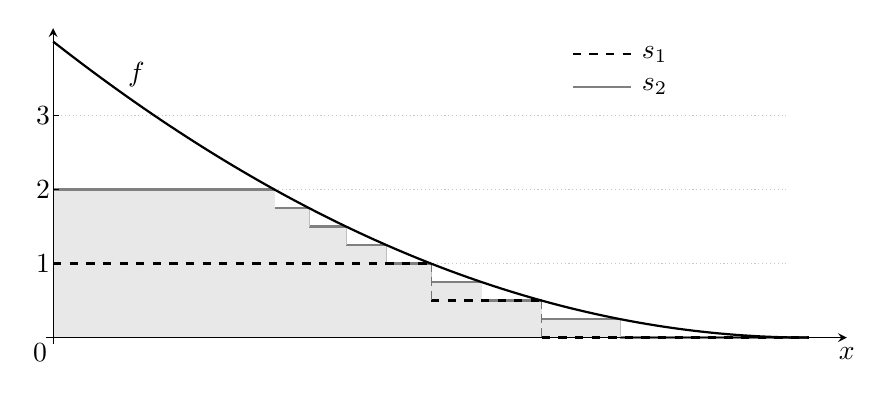
\begin{tikzpicture}[x=1.2cm,y=0.94cm,>=stealth,
                    approximant/.style={line width=0.85pt}]
  \draw[black!22,densely dotted] (0,1) -- (7.75,1);
  \draw[black!22,densely dotted] (0,2) -- (7.75,2);
  \draw[black!22,densely dotted] (0,3) -- (7.75,3);

  % Punkty przecięcia krzywej z poziomami siatki obu przybliżeń.
  \foreach \k in {0,...,7} {
    \pgfmathsetmacro{\level}{\k/4}
    \pgfmathsetmacro{\leftx}{8-4*sqrt((\k+1)/4)}
    \pgfmathsetmacro{\rightx}{8-4*sqrt(\k/4)}
    \fill[black!9] (\leftx,0) rectangle (\rightx,\level);
    \draw[black!50,approximant] (\leftx,\level) -- (\rightx,\level);
    \draw[black!25] (\leftx,\level) -- (\leftx,{\level+1/4});
  }
  \pgfmathsetmacro{\cutoff}{8-4*sqrt(2)}
  \fill[black!9] (0,0) rectangle (\cutoff,2);
  \draw[black!50,approximant] (0,2) -- (\cutoff,2);

  \draw[approximant,dashed] (0,1) -- (4,1);
  \draw[approximant,dashed] (4,1/2) -- ({8-4*sqrt(1/2)},1/2);
  \draw[approximant,dashed] ({8-4*sqrt(1/2)},0) -- (8,0);
  \draw[black!55,densely dashed] (4,1) -- (4,1/2)
    ({8-4*sqrt(1/2)},1/2) -- ({8-4*sqrt(1/2)},0);

  \draw[->,thin] (-0.08,0) -- (8.4,0) node[below] {$x$};
  \draw[->,thin] (0,-0.08) -- (0,4.18);
  \foreach \level in {1,2,3} {
    \draw[thin] (-0.06,\level) -- (0.06,\level)
      node[left=2pt,fill=white,inner sep=1pt] {$\level$};
  }
  \node[below left,inner sep=2pt] at (0,0) {$0$};
  \draw[thick] plot[domain=0:8,samples=85] (\x,{4*(1-\x/8)^2});
  \node[above right,inner sep=2pt] at (0.73,3.31) {$f$};

  \draw[approximant,dashed] (5.5,3.83) -- (6.12,3.83)
    node[right] {$s_1$};
  \draw[black!50,approximant] (5.5,3.39) -- (6.12,3.39)
    node[right,text=black] {$s_2$};
\end{tikzpicture}
\end{document}
